\documentclass[conference]{IEEEtran}
\IEEEoverridecommandlockouts
\usepackage[T1]{fontenc}
\usepackage{cite}
\usepackage{amsmath,amssymb,amsfonts}
\usepackage{graphicx}
\usepackage{booktabs}
\usepackage{textcomp}
\usepackage{xcolor}
\usepackage[hidelinks]{hyperref}
\graphicspath{{figures/}}

\newcommand{\E}{\mathbb{E}}
\newcommand{\Var}{\mathrm{Var}}

\begin{document}

\title{PRISM: Probabilistic Retail Inventory Forecasting\\with State-Space and Machine Learning Models\\
{\large Phase~1 --- Local Kalman Filtering vs.\ Global Gradient Boosting on M5}}

\author{
\IEEEauthorblockN{Member 1, Member 2, Member 3, Member 4, Member 5}
\IEEEauthorblockA{\textit{Newton School of Technology, Rishihood University}\\
Course project: Machine Learning (Phase~1)}
}

\maketitle

\begin{abstract}
Retail inventory decisions need demand forecasts with calibrated uncertainty for many short, sparse and censored sales series. We compare a \emph{local} model, a structural Kalman filter estimated independently for every stock-keeping unit (SKU), with a \emph{global} gradient-boosted model trained jointly on all SKUs, together with seasonal-naive and TSB baselines. The comparison uses 1{,}500 item-store series from the M5 Forecasting Accuracy data. All models produce seven predictive quantiles and are evaluated on an identical rolling-origin backtest (5 origins $\times$ 28 days). Stockouts are \emph{marked} by a backward-looking zero-run test rather than imputed; the filter treats them as missing observations and the global model drops them from its loss. A simulated cold-start cohort measures how each model behaves with 7--168 days of history. The from-scratch filter matches \texttt{statsmodels} to $10^{-9}$ and fits all SKUs in under a minute through a vectorised profile-likelihood search. Both learned models cut WAPE by about 23--25\% relative to seasonal naive. The global LightGBM model is best on every metric (stockout-masked WAPE 0.569, scaled pinball loss 0.264 vs.\ 0.582 and 0.280 for the filter; Diebold--Mariano $p<10^{-20}$). Its advantage grows from about 3\% on smooth series to 9\% on intermittent series and 19\% for items with under two weeks of history, where the local filter's 90\% intervals cover only 71\% of outcomes. These results locate the gap that motivates Phase~2: a global probabilistic network, and a hybrid that feeds Kalman states into it.
\end{abstract}

\begin{IEEEkeywords}
demand forecasting, Kalman filter, state-space models, gradient boosting, quantile regression, intermittent demand, stockouts, cold start, M5
\end{IEEEkeywords}

% =====================================================================
\section{Introduction}
Every stocking decision for a retail SKU rests on a forecast of its demand distribution. The mean is not enough: safety stock depends on an upper quantile. Retail demand is hard to forecast for three reasons. Most item-store series are \emph{intermittent}, with long runs of zeros. Sales are \emph{censored} by stockouts, so a recorded zero may mean that nothing was on the shelf rather than that nobody wanted the item. And assortments change, so many items have \emph{little or no history}.

Two modelling philosophies address these problems differently. \emph{Local} models, such as exponential smoothing and state-space models, fit each series separately. They adapt quickly and have a clean probabilistic interpretation, but they cannot borrow strength across items. \emph{Global} models fit one function to all series~\cite{montero2021,januschowski2020}. They can transfer seasonal, promotional and calendar patterns to sparse and new items, at the cost of careful feature engineering. Global gradient-boosted trees won the M5 accuracy competition~\cite{makridakis2022accuracy}.

This report covers Phase~1 (machine learning) of a two-phase project. We build a fair, leakage-free comparison between a local Kalman filter~\cite{kalman1960} and a global LightGBM model~\cite{ke2017} and measure \emph{where} the local approach falls short. That gap is what the global deep model (DeepAR~\cite{salinas2020}) and the hybrid of Phase~2 are meant to fill. Our contributions are:
\begin{itemize}
\item a from-scratch, vectorised Kalman filter for a structural model with profile-likelihood MLE per SKU, exact missing-data handling for stockouts, and exact quantile back-transformation, verified against \texttt{statsmodels};
\item a horizon-safe \emph{direct} global LightGBM model with Tweedie and quantile losses, whose no-leakage property is unit-tested;
\item a stockout-marking rule that uses only past data, a simulated cold-start cohort, and an evaluation that reports raw and stockout-masked results by horizon, demand class and history length, with significance tests;
\item a reproducible pipeline (one configuration file, cached backtests, generated tables and figures) whose model interface Phase~2 models can use unchanged.
\end{itemize}

% =====================================================================
\section{Literature Review}
\label{sec:lit}
\textbf{State-space models and the Kalman filter.} Kalman~\cite{kalman1960} derived the recursive minimum-variance estimator of the state of a linear Gaussian system. For forecasting, Harvey's structural time-series models~\cite{harvey1989} decompose a series into level, trend and seasonal components, each a state with its own disturbance. Durbin and Koopman~\cite{durbin2012} give the modern treatment: the prediction-error decomposition of the likelihood, concentrating out a scale parameter, diffuse initialisation, and the exact handling of missing observations by skipping the update step. The steady-state filter of the local-level model is simple exponential smoothing~\cite{hyndman2021fpp}, so the filter is the probabilistic foundation of the most widely used retail forecasting methods.

\textbf{Intermittent demand.} Croston~\cite{croston1972} smooths non-zero demand sizes and inter-demand intervals separately. Syntetos and Boylan analyse its bias~\cite{syntetos2005accuracy} and, with Croston, propose the ADI/CV$^2$ classification of demand patterns into smooth, erratic, intermittent and lumpy~\cite{syntetos2005categorization}. TSB~\cite{teunter2011} smooths the demand \emph{probability} every period, so forecasts decay for items that stop selling. Snyder et al.~\cite{snyder2012} and Seeger et al.~\cite{seeger2016} propose count state-space models. Seeger et al.\ also argue for treating stockout periods as missing, the principle we adopt.

\textbf{Global models and gradient boosting.} Gradient boosting~\cite{friedman2001} and its histogram-based implementation LightGBM~\cite{ke2017} dominate tabular forecasting. In M5, most top solutions were global LightGBM models on lag features with a Tweedie loss~\cite{makridakis2022accuracy,jorgensen1987}, and the uncertainty track was won with quantile models~\cite{makridakis2022uncertainty}. Montero-Manso and Hyndman~\cite{montero2021} show that global models are at least as expressive as local ones for any set of series, and that they can afford much richer models because their complexity is supported by the whole collection. Multi-step forecasts can be \emph{recursive} or \emph{direct}~\cite{taieb2012}. Direct models avoid error accumulation and train-test mismatch.

\textbf{Probabilistic forecasting and evaluation.} Proper scoring rules reward calibration and sharpness together~\cite{gneiting2007}. The pinball loss~\cite{koenker1978} is the consistent scoring function for a quantile, and its average over levels approximates the CRPS. Gneiting~\cite{gneiting2011} shows that a point forecast should be evaluated with a scoring function consistent for the functional it targets: absolute error for the median, squared error for the mean. Hyndman and Koehler~\cite{hyndman2006} introduce scaled errors (MASE), the basis of M5's RMSSE. Rolling-origin evaluation~\cite{tashman2000} and the Diebold--Mariano test~\cite{diebold1995} with HAC variance~\cite{newey1987} are standard for comparing forecasters.

\textbf{Deep global models (Phase~2).} DeepAR~\cite{salinas2020} trains one autoregressive recurrent network on all series with a count likelihood and item embeddings, and samples predictive paths. It is the natural deep counterpart of the global model studied here.

% =====================================================================
\section{Data}
\label{sec:data}
\subsection{M5 and the experimental sample}
M5 contains daily unit sales of 3{,}049 products in 10 Walmart stores (CA, TX, WI), 30{,}490 series over 1{,}941 days (2011-01-29 to 2016-05-22). It also includes a calendar with events and state-specific SNAP days, and weekly sell prices. Integrity checks found no missing or negative sales, no duplicate series and a contiguous calendar. The difficulties lie in what the zeros \emph{mean}, not in formatting.

We use one store per state (CA\_1, TX\_1, WI\_1) and 500 series per store. Series are sampled \emph{balanced} over category $\times$ Syntetos--Boylan class~\cite{syntetos2005categorization} (water-filling allocation), with the classes computed only from data before the first forecast origin to avoid selection leakage. The 1{,}500 series comprise 325 smooth, 221 erratic, 482 intermittent and 469 lumpy series (Fig.~\ref{fig:classes}). A series is considered live from its first recorded sale, the convention M5 uses for scaling.

\subsection{Exploratory findings}
The median series has zero sales on 63\% of its active days, and two thirds of all series are zero on more than half of them. Weekly seasonality is strong and stable: Saturdays and Sundays sell about 25\% above the average day (Fig.~\ref{fig:season}). All stores close on Christmas Day. SNAP days lift FOODS sales by 10\% (CA), 16\% (TX) and 6\% (WI). National holidays reduce sales by about 16\%. Prices change in only about 1\% of item-weeks. These findings determine the design: a seasonal state and day-of-week features; a log scale, a Tweedie loss and an intermittent-demand baseline; known-ahead price, event and SNAP features; and explicit handling of non-demand zeros.

\begin{figure}[t]
\centering
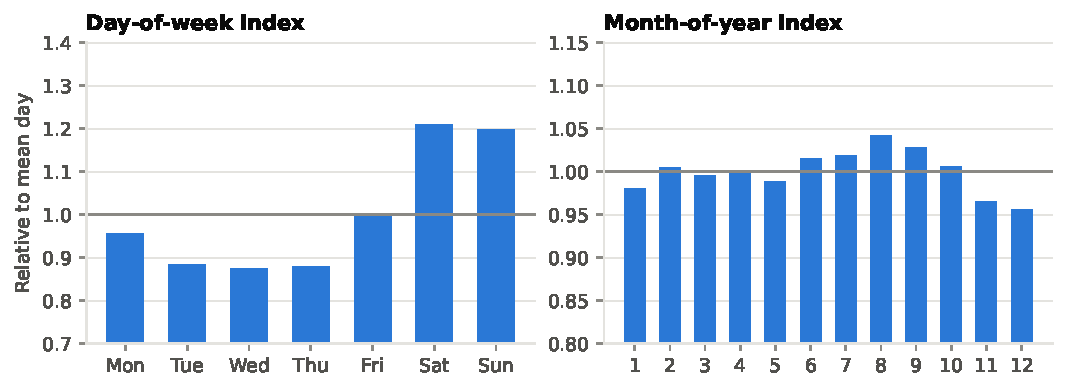
\includegraphics[width=\columnwidth]{eda_seasonality.pdf}
\caption{Day-of-week and month-of-year sales indices (all M5 stores).}
\label{fig:season}
\end{figure}

\begin{figure}[t]
\centering
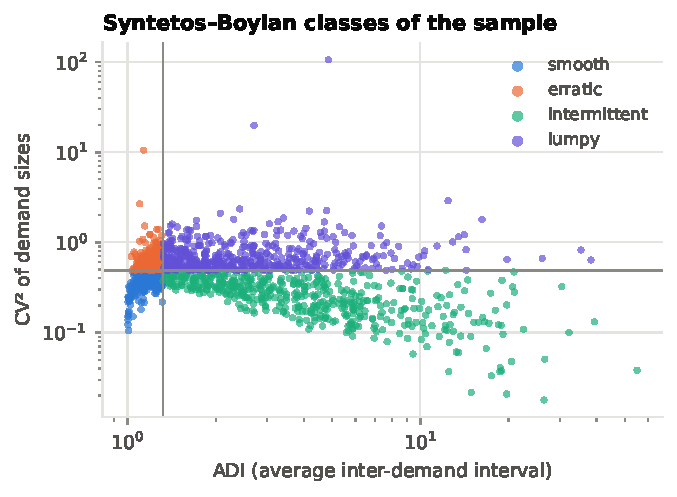
\includegraphics[width=0.8\columnwidth]{eda_demand_classes.pdf}
\caption{Syntetos--Boylan classes of the 1{,}500 sampled series (cut-offs ADI = 1.32, CV$^2$ = 0.49).}
\label{fig:classes}
\end{figure}

\subsection{Stockout marking}
M5 has no inventory data, so stockouts must be inferred. For a zero-run of length $L$ starting at day $s$, let $\hat\pi_0 = (\#\text{zeros}+1)/(W+2)$ be the Laplace-smoothed zero-day rate over the last $W=56$ observed, unflagged days before $s$. The run is flagged as a likely stockout when
\begin{equation}
\hat\pi_0^{\,L} < p^\ast = 10^{-3}.
\end{equation}
The rule looks only backwards from the start of a run. At a forecast origin, a run still in progress is judged on its truncated length, which a unit test confirms equals recomputation from truncated data. The minimum flagged run adapts to the item: three days for an item that is almost never at zero ($\pi_0=0.05$), 31 days for one at zero 80\% of the time. Overall 13.7\% of observed days are flagged: 4.6\% for smooth and 17\% for intermittent series, and only a quarter to a half of all zeros (Fig.~\ref{fig:stockout}). As $p^\ast$ ranges over $10^{-5}$ to $10^{-2}$, the flagged share ranges from 10\% to 18\%. Flags are never used to invent values. They are \emph{marks}: missing data for the filter, excluded rows for the global model's loss, skipped values for the baselines, and a second evaluation view.

\begin{figure}[t]
\centering
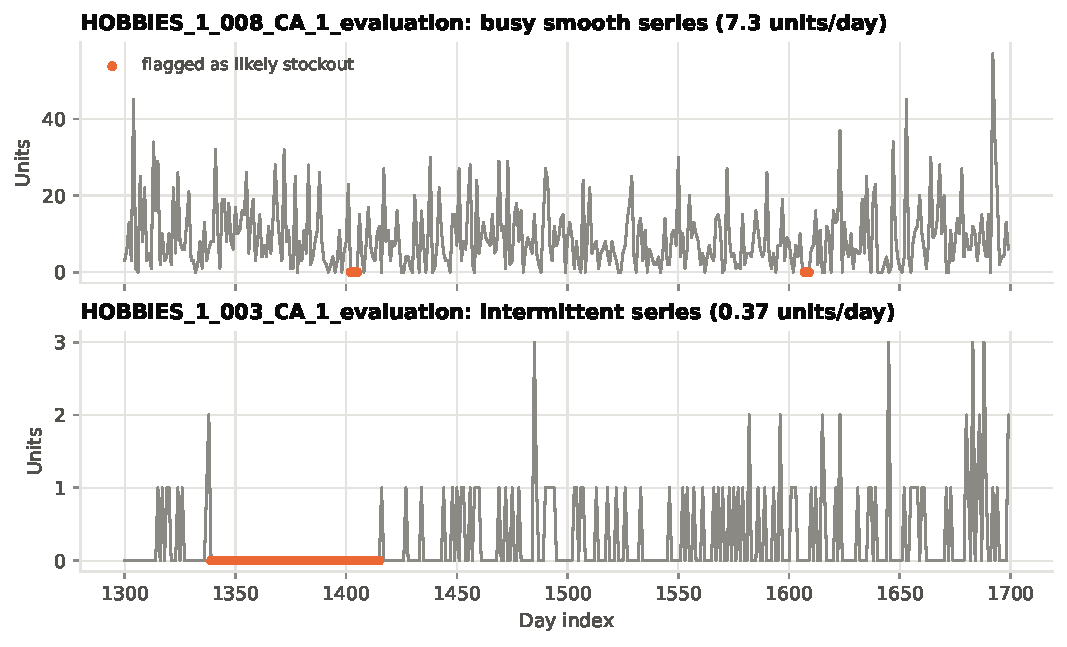
\includegraphics[width=\columnwidth]{stockout_examples.pdf}
\caption{Flagged zero-runs on a busy and an intermittent series. The same rule requires a much longer run on the intermittent item.}
\label{fig:stockout}
\end{figure}

\subsection{Cold start}
Real launches near the backtest period are rare in M5 (three in our sample). We therefore \emph{simulate} 150 new items (10\%): established series whose history before $T_1-L$ is hidden, with $L\in\{7,14,28,56\}$ days and $T_1$ the first origin. Across the five origins these series are seen with 7 to 168 days of history. To keep the hidden history from leaking back, the cross-store features of every series are computed from the full data \emph{minus the series' own raw sales}. A (series, origin) cell with fewer than 90 days of history is labelled cold start, and cells with fewer than 7 days are not scored.

% =====================================================================
\section{Methods}
\label{sec:methods}
All models implement one interface: given the panel truncated at an origin $T$, they return a mean forecast and the quantiles $\alpha\in\{0.05,0.1,0.25,0.5,0.75,0.9,0.95\}$ for $h=1,\dots,28$. Quantiles are clipped at zero and sorted to remove crossings.

\subsection{Baselines}
\emph{Seasonal naive} forecasts $\hat y_{T+h}$ as the most recent same-weekday value that is not a stockout. Its quantiles add the empirical quantiles of the $k$-week-ahead naive errors ($k=\lceil h/7\rceil$, last 364 days). \emph{TSB}~\cite{teunter2011} updates the demand size $z_t$ (only when $y_t>0$) and the demand probability $p_t$ with $\alpha=\beta=0.1$ and forecasts $p_Tz_T$. Its quantiles come from empirical one-step errors.

\subsection{Local model: structural Kalman filter per SKU}
On $z_t=\log(1+y_t)$ we fit the basic structural model~\cite{harvey1989}
\begin{align}
z_t &= \mu_t + \gamma_t + \varepsilon_t, & \varepsilon_t&\sim N(0,\sigma^2_\varepsilon),\\
\mu_{t+1} &= \mu_t + \eta_t, & \eta_t&\sim N(0,\sigma^2_\eta),\\
\gamma_{t+1} &= -\textstyle\sum_{j=0}^{5}\gamma_{t-j} + \omega_t, & \omega_t&\sim N(0,\sigma^2_\omega),
\end{align}
written in state-space form with the 7-dimensional state $\alpha_t=(\mu_t,\gamma_t,\dots,\gamma_{t-5})^\top$, $z_t=Z\alpha_t+\varepsilon_t$ and $\alpha_{t+1}=T\alpha_t+\xi_t$. Given $a_t=\E[\alpha_t\mid z_{1:t-1}]$ and $P_t=\Var[\alpha_t\mid z_{1:t-1}]$, the Kalman recursions are
\begin{align}
v_t &= z_t - Za_t, \quad F_t = ZP_tZ^\top + \sigma^2_\varepsilon, \quad K_t = P_tZ^\top F_t^{-1},\\
a_{t+1} &= T(a_t + K_tv_t), \quad P_{t+1} = T(P_t - K_tF_tK_t^\top)T^\top + Q.
\end{align}
When $z_t$ is missing (before launch, or a flagged stockout), the update is skipped. This yields the exact conditional distribution, which is why marking rather than imputing fits naturally into the state-space framework.

\textbf{Estimation.} Writing $Q=\sigma^2_\varepsilon\,\mathrm{diag}(q_\eta,q_\omega,0,\dots)$, we run the filter with unit observation variance. Then $\hat\sigma^2_\varepsilon=n^{-1}\sum_t v_t^2/F^\ast_t$ in closed form, and the profile log-likelihood~\cite{durbin2012}
\begin{equation}
\ell_c(q)=-\tfrac n2\big[\log 2\pi+1+\log\hat\sigma^2_\varepsilon\big]-\tfrac12\textstyle\sum_t\log F^\ast_t
\end{equation}
depends only on the two signal-to-noise ratios. We maximise it on a $13\times7$ log-spaced grid followed by a $5\times5$ local refinement. The filter is vectorised \emph{across SKUs}, so a grid point costs one pass over all 1{,}500 series (0.5\,s), and the full per-SKU MLE takes about 50\,s per origin. The initial state is approximately diffuse ($P_1=10^6I$), with the first seven observations excluded from $\ell_c$. The fit uses the last 730 days, and series with fewer than 56 in-stock observations use default ratios. Our implementation reproduces \texttt{statsmodels}' log-likelihood, one-step predictions and $h$-step variances to $10^{-9}$, including with missing data.

\textbf{Forecast distribution.} Iterating the prediction step gives $z_{T+h}\sim N(m_h,s_h^2)$. Quantiles are preserved by monotone maps, so $Q_y(\alpha)=\exp(m_h+s_h\Phi^{-1}(\alpha))-1$ exactly. The mean is the log-normal mean $\exp(m_h+s_h^2/2)-1$. The random-walk level makes $s_h^2$ grow without bound over long horizons and long unobserved gaps (for example a delisted item), and the log-normal mean amplifies this. We therefore cap $s_h^2$ at the series' own marginal variance of $z$: a forecast is never less informative than the unconditional distribution. Items with fewer than 14 in-stock days in the window are filtered on their raw history.

\subsection{Global model: LightGBM on lag features}
One model is trained on all series and days of the last 730 days before the origin, excluding flagged stockout rows. It uses a \emph{horizon-safe direct} design: every sales-derived feature for target day $t$ uses only data up to $t-L$, with $L\ge h$, so the model needs no recursion and cannot see the future. Two variants are trained: $L=7$ serves $h\le7$ and $L=28$ serves $8\le h\le28$; the pure $L=28$ model is kept as an ablation. Features are:
\begin{itemize}
\item lags $L, L{+}1, L{+}2, L{+}7, L{+}14, L{+}21, L{+}28, 364$;
\item rolling mean, standard deviation, maximum and zero share over 7--364 days, the same-weekday mean, momentum, the expanding mean, and the current zero streak;
\item the same item's mean sales in the other nine stores and the department-store mean (own sales excluded);
\item price, relative price and weekly price change;
\item calendar features (day of week, month, week, events, days to and since an event) and SNAP for the series' state;
\item item age and categorical item, department, category, store and state identifiers.
\end{itemize}
Prices and the calendar are known ahead, as in M5. The mean model uses a Tweedie loss (variance power 1.1)~\cite{jorgensen1987}, a compound Poisson--Gamma likelihood with a point mass at zero. Its number of rounds is chosen by early stopping on the last 28 days \emph{of the training window}, after which it is refit on the whole window. Each quantile has its own model trained with the pinball loss~\cite{koenker1978}. A unit test confirms that the feature row for day $t^\ast$ is identical whether the data end at $t^\ast-L$ or at $t^\ast-1$.

% =====================================================================
\section{Experimental Design}
\textbf{Rolling origin.} We use five origins (cutoffs after d\_1801, d\_1829, \dots, d\_1913, 28 days apart), each with a 28-day horizon; the last window is the official M5 test period~\cite{tashman2000}. At every origin each model is refit on a panel physically truncated at the origin, and all models are scored on the same 209{,}860 cells.

\textbf{Metrics.} Following~\cite{gneiting2011}, MAE and WAPE ($\sum|y-\hat y|/\sum y$) are computed on the predictive \emph{median}, and RMSE and RMSSE~\cite{hyndman2006,makridakis2022accuracy} on the predictive \emph{mean}. Probabilistic accuracy is the pinball loss $\rho_\alpha(u)=\max(\alpha u,(\alpha-1)u)$ averaged over the 7 levels, and its scaled version SPL (divided by the series' in-sample one-step naive MAE, as in M5~\cite{makridakis2022uncertainty}). We also report the empirical coverage and width of the 80\% and 90\% intervals. For count data, quantile $\alpha$ is calibrated when $P(y<q_\alpha)\le\alpha\le P(y\le q_\alpha)$.

\textbf{Views and tests.} Results are reported on all target days and on \emph{stockout-masked} days, by horizon bucket, demand class and history length. Differences are tested with the Diebold--Mariano test~\cite{diebold1995} on the daily cross-sectional mean loss (140 days, Newey--West lag 7~\cite{newey1987}) and with a Wilcoxon signed-rank test across series.

% =====================================================================
\section{Results}
\label{sec:results}
\begin{table*}[t]
\centering
\caption{Rolling-origin backtest, 5 origins $\times$ 28 days, 1,500 series. MAE/WAPE use the predictive median, RMSE/RMSSE the mean. Best per column in bold (coverage: closest to nominal).}
\label{tab:overall}
\scriptsize
\setlength{\tabcolsep}{3.5pt}
\resizebox{\ifdim\width>\textwidth \textwidth\else\width\fi}{!}{%
\begin{tabular}{llrrrrrrrrr}
\toprule
Segment & Model & MAE & RMSE & WAPE & RMSSE & Pinball & SPL & Cov80 & Cov90 & Width90 \\
\midrule
All target days & Seasonal naive & 2.100 & 4.092 & 0.844 & 0.969 & 0.612 & 0.356 & 0.857 & 0.923 & 7.024 \\
 & TSB (Croston-type) & 1.668 & 3.275 & 0.670 & 0.742 & 0.498 & 0.275 & 0.778 & 0.878 & 6.495 \\
 & Kalman filter (local) & 1.620 & 3.683 & 0.651 & 0.736 & 0.489 & 0.272 & \textbf{0.803} & 0.892 & 7.469 \\
 & LightGBM (global) & \textbf{1.585} & \textbf{3.166} & \textbf{0.637} & \textbf{0.722} & \textbf{0.464} & \textbf{0.253} & 0.777 & 0.903 & 6.467 \\
 & LightGBM lag-28 only & 1.598 & 3.185 & 0.642 & 0.724 & 0.468 & 0.254 & 0.774 & \textbf{0.902} & 6.482 \\
\midrule
Stockout-masked & Seasonal naive & 2.101 & 4.000 & 0.757 & 0.978 & 0.610 & 0.358 & 0.857 & 0.924 & 7.087 \\
 & TSB (Croston-type) & 1.664 & 3.181 & 0.600 & 0.753 & 0.494 & 0.281 & 0.790 & 0.887 & 6.549 \\
 & Kalman filter (local) & 1.615 & 3.479 & 0.582 & 0.744 & 0.485 & 0.280 & 0.818 & \textbf{0.903} & 7.563 \\
 & LightGBM (global) & \textbf{1.579} & \textbf{3.040} & \textbf{0.569} & \textbf{0.732} & \textbf{0.466} & \textbf{0.264} & \textbf{0.798} & 0.915 & 6.523 \\
 & LightGBM lag-28 only & 1.589 & 3.061 & 0.573 & 0.733 & 0.469 & 0.265 & 0.796 & 0.915 & 6.542 \\
\bottomrule
\end{tabular}
}
\end{table*}

\textbf{Overall (Table~\ref{tab:overall}).} Both learned models improve on seasonal naive by about a quarter: masked WAPE is 0.757 for naive vs.\ 0.582 for Kalman and 0.569 for LightGBM. The global LightGBM model is best on every accuracy metric, with masked SPL 5.6\% below the filter's (0.264 vs.\ 0.280) and a clearly lower RMSE (3.04 vs.\ 3.48). The Kalman filter is the best local method. It beats TSB on WAPE, RMSSE and pinball loss, and its masked 90\% coverage (0.903) is the closest to nominal. Masking stockout days lowers every model's WAPE by roughly 0.07, which confirms that flagged zeros penalise forecasts of genuine demand.

\textbf{Significance (Table~\ref{tab:dm}).} All headline differences are significant. LightGBM vs.\ Kalman gives DM $=-11.2$ on pinball loss ($p<10^{-20}$), with LightGBM ahead on 79\% of series. The short-lag variant beats the lag-28 ablation by a small but significant margin ($p=0.003$), entirely through $h\le7$ (SPL 0.260 vs.\ 0.264).

\begin{table}[t]
\centering
\caption{Diebold--Mariano tests on the daily mean loss (140 target days, HAC lag 7) and the share of series where model A has lower mean loss (Wilcoxon signed-rank $p$). Negative DM: A is better.}
\label{tab:dm}
\scriptsize
\setlength{\tabcolsep}{3pt}
\resizebox{\columnwidth}{!}{%
\begin{tabular}{llrrrr}
\toprule
A vs B & Loss & DM & $p$ & A better & Wilcoxon $p$ \\
\midrule
LightGBM vs Kalman filter & pinball & -11.16 & 4.88e-21 & 79\% & 0 \\
LightGBM vs Kalman filter & abs. error & -6.33 & 3.11e-09 & 72\% & 0 \\
LightGBM vs TSB & pinball & -12.13 & 1.5e-23 & 81\% & 0 \\
LightGBM vs TSB & abs. error & -12.62 & 8.44e-25 & 80\% & 0 \\
Kalman filter vs TSB & pinball & -5.26 & 5.24e-07 & 55\% & 3.6e-13 \\
Kalman filter vs TSB & abs. error & -10.13 & 2.14e-18 & 54\% & 7.7e-13 \\
Kalman filter vs Seasonal naive & pinball & -40.72 & 3.92e-79 & 96\% & 0 \\
Kalman filter vs Seasonal naive & abs. error & -45.25 & 4.71e-85 & 92\% & 0 \\
LightGBM vs LightGBM lag-28 only & pinball & -3.00 & 0.00317 & 58\% & 2.2e-16 \\
LightGBM vs LightGBM lag-28 only & abs. error & -3.06 & 0.00268 & 56\% & 1.9e-12 \\
\bottomrule
\end{tabular}
}
\end{table}

\begin{figure*}[t]
\centering
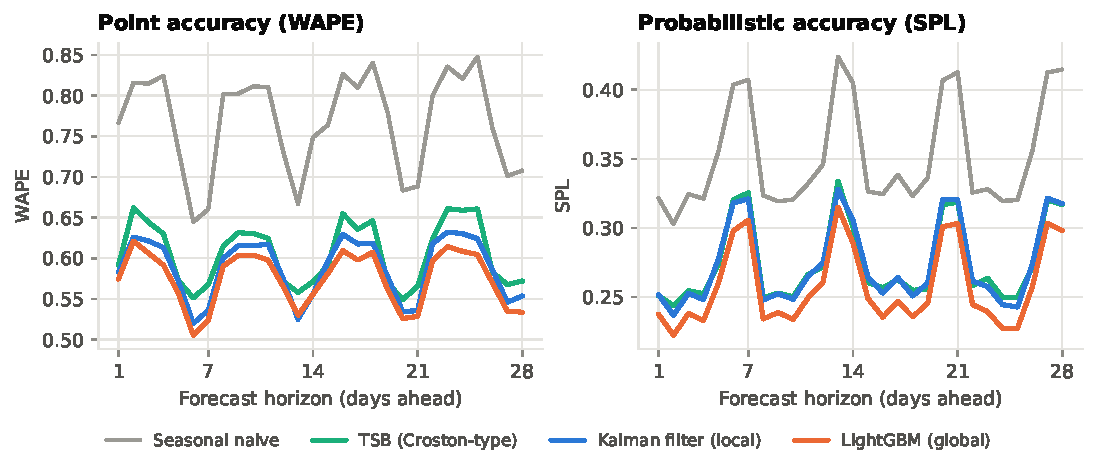
\includegraphics[width=0.85\textwidth]{metric_by_horizon.pdf}
\caption{Stockout-masked WAPE and SPL by horizon. The saw-tooth is the weekly cycle (all origins fall on the same weekday, so weekend horizons carry more volume). The model ranking is the same at every horizon.}
\label{fig:horizon}
\end{figure*}

\textbf{Horizon (Fig.~\ref{fig:horizon}).} Accuracy varies far more with the day of week than with the horizon, and the ranking never changes. Neither local model degrades much over 28 days, because their forecasts are dominated by a stable level and weekly pattern.

\begin{table}[t]
\centering
\caption{Accuracy by Syntetos--Boylan demand class (stockout-masked).}
\label{tab:class}
\scriptsize
\setlength{\tabcolsep}{3.5pt}
\resizebox{\ifdim\width>\columnwidth \columnwidth\else\width\fi}{!}{%
\begin{tabular}{llrrrr}
\toprule
Segment & Model & WAPE & RMSSE & SPL & Cov90 \\
\midrule
erratic & Seasonal naive & 0.762 & 0.907 & 0.299 & 0.911 \\
 & TSB (Croston-type) & 0.600 & 0.715 & 0.246 & 0.892 \\
 & Kalman filter (local) & 0.576 & 0.716 & 0.239 & \textbf{0.896} \\
 & LightGBM (global) & \textbf{0.572} & \textbf{0.693} & \textbf{0.232} & 0.895 \\
\midrule
intermittent & Seasonal naive & 1.038 & 1.053 & 0.416 & 0.940 \\
 & TSB (Croston-type) & 0.813 & 0.797 & 0.322 & 0.879 \\
 & Kalman filter (local) & 0.836 & 0.786 & 0.329 & \textbf{0.902} \\
 & LightGBM (global) & \textbf{0.770} & \textbf{0.784} & \textbf{0.299} & 0.929 \\
\midrule
lumpy & Seasonal naive & 1.046 & 0.947 & 0.379 & 0.919 \\
 & TSB (Croston-type) & 0.798 & 0.715 & 0.286 & \textbf{0.893} \\
 & Kalman filter (local) & 0.787 & 0.710 & 0.285 & 0.913 \\
 & LightGBM (global) & \textbf{0.769} & \textbf{0.703} & \textbf{0.274} & 0.922 \\
\midrule
smooth & Seasonal naive & 0.571 & 0.961 & 0.287 & 0.916 \\
 & TSB (Croston-type) & 0.469 & 0.765 & 0.239 & 0.885 \\
 & Kalman filter (local) & 0.444 & 0.749 & 0.232 & 0.898 \\
 & LightGBM (global) & \textbf{0.439} & \textbf{0.723} & \textbf{0.225} & \textbf{0.900} \\
\bottomrule
\end{tabular}
}
\end{table}

\begin{figure}[t]
\centering
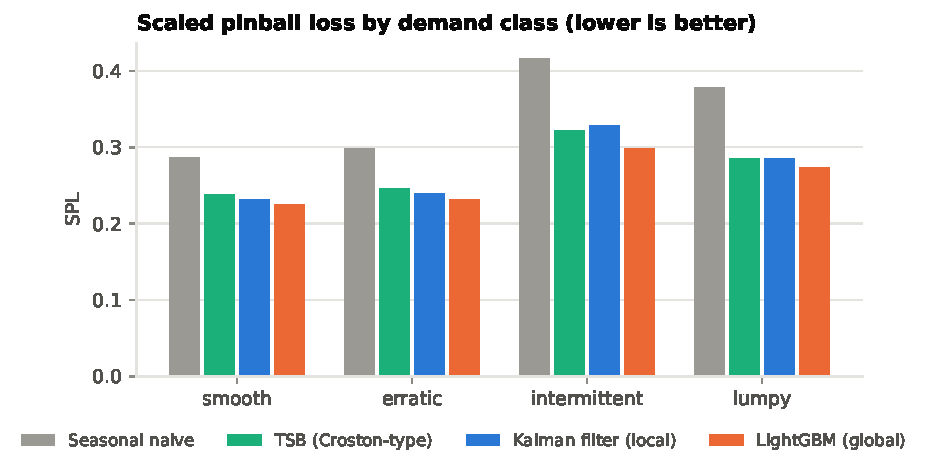
\includegraphics[width=\columnwidth]{spl_by_class.pdf}
\caption{Scaled pinball loss by demand class (stockout-masked).}
\label{fig:class}
\end{figure}

\textbf{Demand class (Table~\ref{tab:class}, Fig.~\ref{fig:class}).} The global model's advantage over the filter grows with sparsity: SPL is 3\% lower on smooth and erratic series, 4\% on lumpy series and 9\% on intermittent series. On intermittent series even TSB beats the filter on WAPE (0.813 vs.\ 0.836). A Gaussian filter on $\log(1+y)$ is a poor description of mostly-zero counts, while the global model pools the zero-inflation structure across hundreds of similar items.

\begin{table}[t]
\centering
\caption{Cold-start vs established series (stockout-masked).}
\label{tab:coldstart}
\scriptsize
\setlength{\tabcolsep}{3.5pt}
\resizebox{\ifdim\width>\columnwidth \columnwidth\else\width\fi}{!}{%
\begin{tabular}{llrrrrr}
\toprule
Segment & Model & n & WAPE & RMSSE & SPL & Cov90 \\
\midrule
Cold start ($<$90 days) & Seasonal naive & 10,966 & 0.768 & 1.097 & 0.394 & \textbf{0.884} \\
 & TSB (Croston-type) & 10,966 & 0.621 & 0.862 & 0.312 & 0.859 \\
 & Kalman filter (local) & 10,966 & 0.645 & 0.952 & 0.328 & 0.847 \\
 & LightGBM (global) & 10,966 & \textbf{0.615} & \textbf{0.851} & \textbf{0.286} & 0.879 \\
\midrule
Established & Seasonal naive & 177,297 & 0.757 & 0.971 & 0.356 & 0.926 \\
 & TSB (Croston-type) & 177,297 & 0.598 & 0.746 & 0.279 & 0.888 \\
 & Kalman filter (local) & 177,297 & 0.578 & 0.732 & 0.277 & \textbf{0.907} \\
 & LightGBM (global) & 177,297 & \textbf{0.566} & \textbf{0.725} & \textbf{0.263} & 0.917 \\
\bottomrule
\end{tabular}
}
\end{table}

\begin{figure*}[t]
\centering
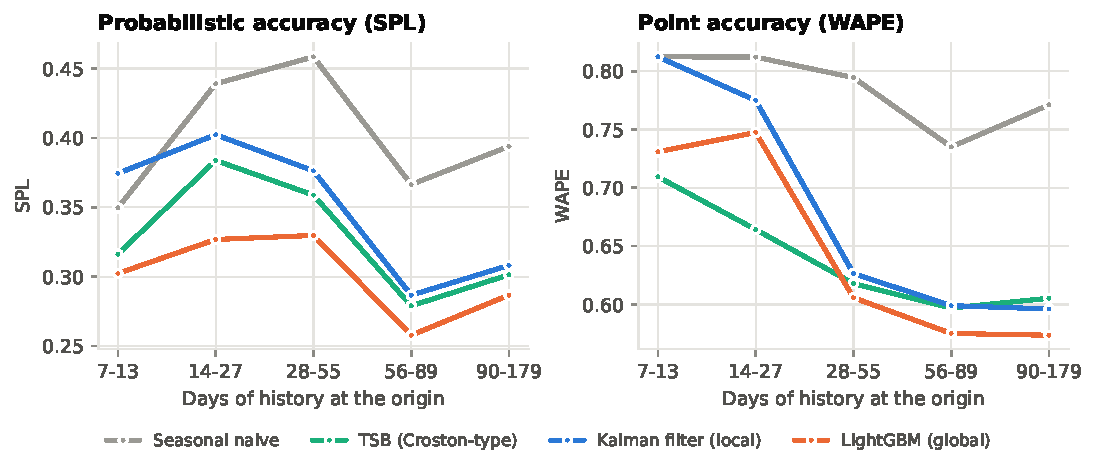
\includegraphics[width=0.85\textwidth]{cold_start_curve.pdf}
\caption{Learning curves of the simulated new items: stockout-masked SPL and WAPE vs.\ days of history at the origin.}
\label{fig:cold}
\end{figure*}

\textbf{Cold start (Table~\ref{tab:coldstart}, Fig.~\ref{fig:cold}).} Here the gap is largest. On cold-start cells LightGBM's SPL is 13\% below the filter's (0.286 vs.\ 0.328), compared with 5\% on established cells. With 7--13 days of history the filter's SPL is 0.374 vs.\ 0.302 (19\%), and its 90\% interval covers only 71\% of outcomes, while LightGBM's covers 90\%. With so little data the local MLE cannot estimate its own noise, so it is over-confident. The global model draws on the same item in other stores, the department and the learned price and calendar effects. As history accumulates the filter recovers quickly, and its gap closes to about 10\% by 56--89 days.

\begin{figure}[t]
\centering
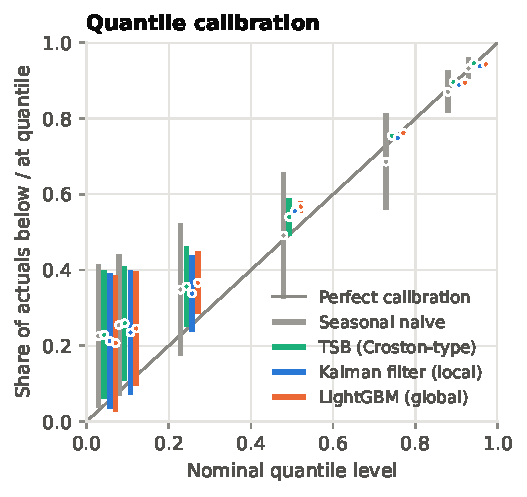
\includegraphics[width=0.85\columnwidth]{calibration.pdf}
\caption{Quantile calibration for count data. Each bar is $[P(y<q_\alpha),P(y\le q_\alpha)]$; a quantile is calibrated when its bar crosses the diagonal.}
\label{fig:calib}
\end{figure}

\textbf{Calibration (Fig.~\ref{fig:calib}).} Lower quantiles are calibrated for all models; their intervals are long because of the point mass at zero. Upper quantiles of the filter and LightGBM fall slightly short (0.889 and 0.895 of outcomes below the 0.9 quantile). Seasonal naive reaches nominal coverage only through wide intervals, at a 30\% higher pinball loss, which illustrates why coverage alone is not a sufficient criterion~\cite{gneiting2007}.

\begin{figure*}[t]
\centering
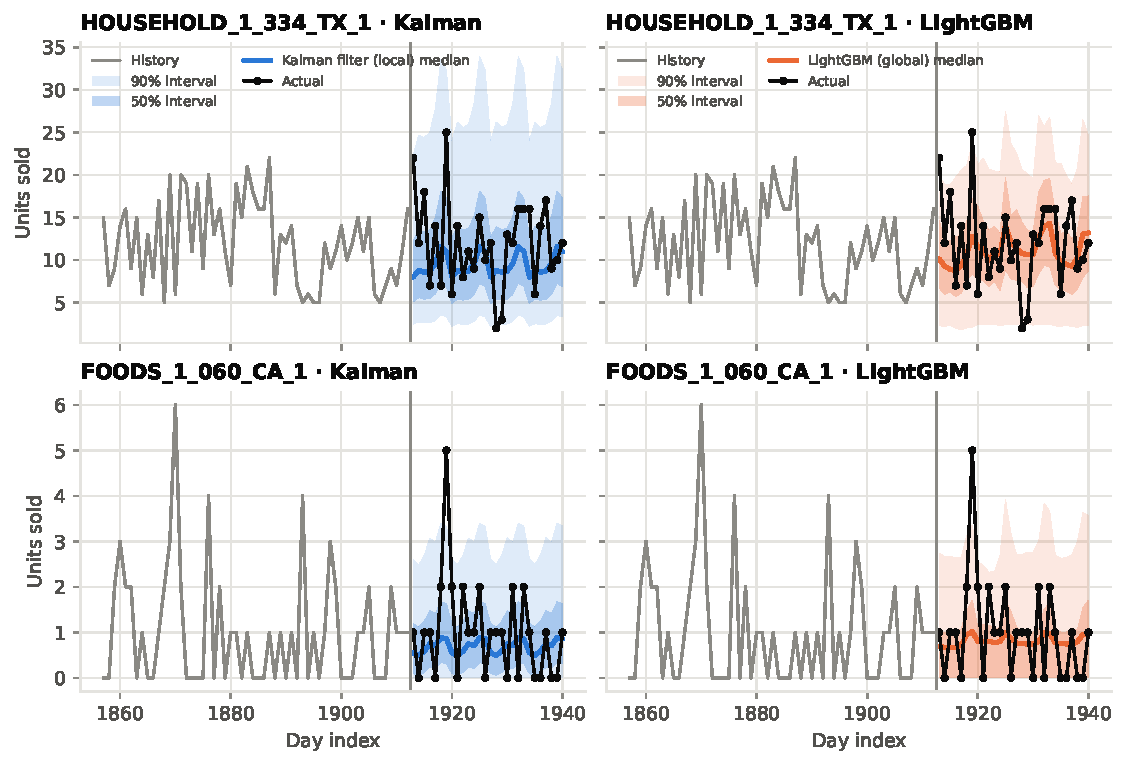
\includegraphics[width=0.85\textwidth]{fan_charts.pdf}
\caption{Forecasts at the last origin (the M5 test window) for a smooth (top) and an intermittent (bottom) series: Kalman filter (left) vs.\ LightGBM (right), with 50\% and 90\% intervals.}
\label{fig:fan}
\end{figure*}

\textbf{Examples (Fig.~\ref{fig:fan}).} On the smooth series both models track the weekly pattern. LightGBM's median is closer to the realised level (11.1 vs.\ 9.5 units against an average of 12), and its upper tail is tighter (95\% quantile 21.9 vs.\ 27.8). On the intermittent series LightGBM's lower quartile is exactly zero, a point mass learned from many similar items, while the filter's continuous log-normal band stays above zero (0.2).

\textbf{Cost.} Per origin, the vectorised filter fits 1{,}500 per-SKU MLEs in about 51\,s. LightGBM's 18 boosters (2 horizon variants $\times$ (1 mean + 7 quantile) models, plus 2 early-stopping runs) take about 130\,s on an 8-core laptop.

% =====================================================================
\section{Discussion}
\textbf{The local--global gap.} The results support the hypothesis behind the project. A local filter adapts quickly and needs no feature engineering. Its intervals are well calibrated once a series has a few months of history, and its treatment of stockouts is exact. But it learns each series in isolation, so it is weakest exactly where inventory risk is highest: sparse and new items. In those cases the global model's ability to transfer patterns gives the largest gains in both accuracy and calibration. The gains are consistent (79\% of series) yet moderate overall (about 6\% SPL), which suggests the two approaches are complementary rather than substitutes.

\textbf{Limitations.} The stockout rule assumes independent zero days and cannot distinguish a stockout from a delisting; we mitigate this with a sensitivity analysis and by always reporting unmasked metrics. The filter's Gaussian log-scale observation model fits intermittent counts poorly. Cold start is simulated, although the hidden history cannot leak. The sample covers three of the ten stores, and hyperparameters were set once rather than tuned per origin.

\textbf{Phase~2.} The same harness, metrics and segments will evaluate (i)~a global DeepAR model~\cite{salinas2020} with a negative-binomial likelihood, item embeddings and calendar/price covariates; and (ii)~a \emph{hybrid} that feeds the Kalman filter's filtered level, seasonal effect and state variance to the network as dynamic covariates. The hybrid combines fast local adaptation with global sharing, and ablations with and without the Kalman features will test its value.

% =====================================================================
\section{Conclusion}
PRISM delivers a leakage-free, reproducible comparison of local and global probabilistic demand forecasters on M5. It includes a verified from-scratch Kalman filter, a horizon-safe global LightGBM model, principled stockout marking and an explicit cold-start evaluation. The global model wins consistently and significantly, most of all on intermittent and new items, while the local filter remains the strongest and best-calibrated local method. Measuring that gap is the starting point for Phase~2.

\section*{Reproducibility and Contributions}
All code, configuration and notebooks are in the project repository. \texttt{make data backtest assets} regenerates every number, table and figure in this report (about 20 minutes on a laptop), and 18 unit tests cover the metrics, the filter (against \texttt{statsmodels}), leakage, stockout flags and backtest alignment. Module ownership: data and EDA (M1), stockouts and cold start (M2), Kalman filter and baselines (M3), features and LightGBM (M4), evaluation and reporting (M5).

\bibliographystyle{IEEEtran}
\bibliography{refs}

\end{document}
